\documentclass[10pt]{beamer}
\usetheme{metropolis}
\usepackage{booktabs}
\usepackage{tabularx}
\usepackage{calc}
\usepackage{tikz}

% Setup for faculty images
\newlength{\imageheight}
\setlength{\imageheight}{3.5cm}

% Define CSUF brand colors
\definecolor{titanblue}{HTML}{00244E}
\definecolor{mediumblue}{HTML}{0F3F8C}
\definecolor{skyblue}{HTML}{EBFBFF}
\definecolor{titanorange}{HTML}{FF7900}
\definecolor{titangray}{HTML}{F5F5F5}
\definecolor{titantext}{HTML}{222222}

% Customize metropolis theme colors
\setbeamercolor{normal text}{fg=titantext, bg=white}
\setbeamercolor{alerted text}{fg=titanorange}
\setbeamercolor{example text}{fg=mediumblue}

% Title page colors
\setbeamercolor{title}{fg=titanblue, bg=white}
\setbeamercolor{subtitle}{fg=mediumblue, bg=white}
\setbeamercolor{institute}{fg=titanorange, bg=white}
\setbeamercolor{date}{fg=titanblue, bg=white}

% Frame title colors
\setbeamercolor{frametitle}{fg=white, bg=titanblue}
\setbeamercolor{framesubtitle}{fg=mediumblue, bg=white}

% Block environment colors
\setbeamercolor{block title}{fg=white, bg=titanblue}
\setbeamercolor{block body}{fg=titantext, bg=skyblue!10}

% Item colors
\setbeamercolor{itemize item}{fg=titanorange}
\setbeamercolor{itemize subitem}{fg=mediumblue}
\setbeamercolor{itemize subsubitem}{fg=titanblue}

% Footer and header colors
\setbeamercolor{footer}{fg=titantext}
\setbeamercolor{header}{fg=titanblue}

% Customize fonts
\setbeamerfont{title}{size=\Large, series=\bfseries}
\setbeamerfont{frametitle}{size=\large, series=\bfseries}

% Simple title page template
\defbeamertemplate*{title page}{customized}[1][]
{
\vspace{1cm}
 {\usebeamerfont{title}\usebeamercolor[fg]{title}\inserttitle\par}
\vspace{0.5cm}
 {\usebeamerfont{subtitle}\usebeamercolor[fg]{subtitle}\insertsubtitle\par}
\vspace{0.5cm}
 {\usebeamerfont{date}\usebeamercolor[fg]{date}\insertdate\par}
\vfill
 {\insertinstitute\par}
}

% Add progress bar
\makeatletter
\setbeamertemplate{headline}{%
\begin{beamercolorbox}[wd=\paperwidth,ht=0.4cm,dp=0cm]{titanblue}%
\begin{tikzpicture}
\fill[titanorange] (0,0) rectangle (\the\paperwidth*\insertframenumber/\inserttotalframenumber,0.4cm);
\end{tikzpicture}%
\end{beamercolorbox}%
}
\makeatother

\begin{document}

\title{From Ancient Ideas to Modern Governance}
\subtitle{Political Theory and Policy\\POSC 315: Introduction to Public Policy\\Lecture 1 (Part 2 of 3)}
\date{}
\institute{California State University, Fullerton}

\maketitle

% Introduction to Political Theory
\begin{frame}
\frametitle{Political Theory, Quickly}

\begin{block}{}
\centering
Political theory is the study of the ideas and values that underpin political systems and institutions.
\end{block}

\pause
\vspace{0.5cm}
\textbf{Why Political Theory Matters for Public Policy:}
\begin{itemize}
\item Provides a foundation for understanding governance
\item Reveals competing values in policy debates
\item Helps us understand the purpose of policy
\item Frames how we conceptualize problems and solutions
\end{itemize}

\end{frame}

% Early Concepts
\begin{frame}
\frametitle{Early Concepts: Gilgamesh}
\framesubtitle{2500-ish BCE}

\begin{itemize}
\item<1-> One of the earliest written records of governance
\item<2-> Introduces the concept of two classes: rulers and subjects
\item<3-> Sets the stage for Western ideas about hierarchy and authority
\end{itemize}

\end{frame}

% Greek Foundations
\begin{frame}
\frametitle{The Greeks: Foundations of Political Philosophy}
\framesubtitle{6th-3rd Century BCE}

\begin{columns}
\begin{column}{0.32\textwidth}
\begin{block}{Socrates}
\pause
Ethics and justice in governance
\end{block}
\end{column}

\begin{column}{0.32\textwidth}
\begin{block}{Plato}
\pause
The ``ideal state'' ruled by philosopher-kings
\end{block}
\end{column}

\begin{column}{0.32\textwidth}
\begin{block}{Aristotle}
\pause
Empirical approach to politics; governments must promote virtue and balance
\end{block}
\end{column}
\end{columns}

\end{frame}

% Renaissance & Early Modern Thinkers
\begin{frame}
\frametitle{Renaissance \& Early Modern Thinkers}
\framesubtitle{15th-17th Century}

\begin{columns}
\begin{column}{0.48\textwidth}
\begin{block}{Machiavelli}
\pause
Politics as power; pragmatism over idealism

\vspace{0.3cm}
\textcolor{mediumblue}{\textit{The Prince} (1513)}
\end{block}
\end{column}

\begin{column}{0.48\textwidth}
\begin{block}{Bacon}
\pause
Knowledge as power; science and governance intertwined

\vspace{0.3cm}
\textcolor{mediumblue}{\textit{New Atlantis} (1627)}
\end{block}
\end{column}
\end{columns}

\end{frame}

% The Enlightenment
\begin{frame}
\frametitle{The Enlightenment}
\framesubtitle{17th-18th Centuries}

\begin{columns}
\begin{column}{0.48\textwidth}
\begin{block}{Hobbes}
\pause
Social contract; strong authority prevents chaos

\vspace{0.2cm}
\textcolor{mediumblue}{\textit{Leviathan} (1651)}
\end{block}

\vspace{0.3cm}

\begin{block}{Rousseau}
\pause
General will; collective good over individual interests

\vspace{0.2cm}
\textcolor{mediumblue}{\textit{Social Contract} (1762)}
\end{block}
\end{column}

\begin{column}{0.48\textwidth}
\begin{block}{Locke}
\pause
Rights to life, liberty, and property; government must protect individual freedoms

\vspace{0.2cm}
\textcolor{mediumblue}{\textit{Two Treatises} (1689)}
\end{block}

\vspace{0.3cm}

\begin{block}{Montesquieu}
\pause
Separation of powers to avoid tyranny

\vspace{0.2cm}
\textcolor{mediumblue}{\textit{Spirit of Laws} (1748)}
\end{block}
\end{column}
\end{columns}

\end{frame}

% The American Regime
\begin{frame}
\frametitle{The American Regime}
\framesubtitle{18th-19th Centuries}

\begin{block}{}
\begin{itemize}
\item<1-> \textbf{Founding Fathers:} Jefferson, Madison, and Hamilton synthesized Enlightenment ideals for the U.S. context
\item<2-> Key principles: liberty, equality, and a government of the people
\item<3-> Continuing influence: Lincoln, Roosevelt(s), King, and others, interpreting liberalism in different eras
\end{itemize}
\end{block}

\pause
\vspace{0.5cm}
\centering
These ideals continue to shape American policy debates today

\end{frame}

% 20th Century Theorists
\begin{frame}
\frametitle{20th Century Theorists}

\begin{columns}
\begin{column}{0.48\textwidth}
\begin{block}{Rawls}
\pause
Justice as fairness; prioritizing the least advantaged
\end{block}

\vspace{0.3cm}

\begin{block}{Dewey}
\pause
Pragmatism and the role of public engagement in policy
\end{block}
\end{column}

\begin{column}{0.48\textwidth}
\begin{block}{Marx \& Weber}
\pause
Economic forces and power dynamics shape society
\end{block}

\vspace{0.3cm}

\begin{block}{Lasswell}
\pause
``Who gets what, when, and how''---the essence of politics
\end{block}
\end{column}
\end{columns}

\end{frame}

% Classical Liberalism
\begin{frame}
\frametitle{The Evolution of Liberalism}

Liberalism evolves as a response to changing societal needs and economic conditions:

\vspace{0.5cm}

\begin{center}
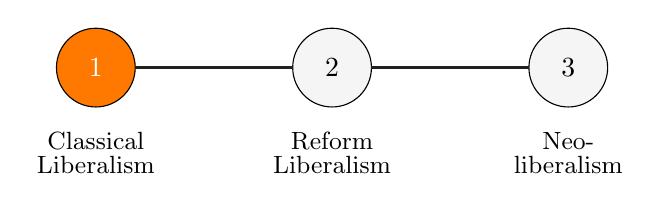
\begin{tikzpicture}
\node[draw, circle, fill=titanorange, text=white, minimum size=1cm] at (0,0) {1};
\node[draw, circle, fill=titangray, minimum size=1cm] at (3,0) {2};
\node[draw, circle, fill=titangray, minimum size=1cm] at (6,0) {3};

\draw[thick, titantext] (0.5,0) -- (2.5,0);
\draw[thick, titantext] (3.5,0) -- (5.5,0);

\node[below] at (0,-0.7) {\small Classical};
\node[below] at (0,-1.0) {\small Liberalism};
\node[below] at (3,-0.7) {\small Reform};
\node[below] at (3,-1.0) {\small Liberalism};
\node[below] at (6,-0.7) {\small Neo-};
\node[below] at (6,-1.0) {\small liberalism};
\end{tikzpicture}
\end{center}

\vspace{0.5cm}

\begin{block}{Classical Liberalism}
Rooted in the Enlightenment, emphasizing individual freedoms, limited government, and free markets

\vspace{0.3cm}
\textcolor{mediumblue}{\textit{18th - 19th Century}}
\end{block}

\end{frame}

% Reform Liberalism
\begin{frame}
\frametitle{The Evolution of Liberalism}

\begin{center}
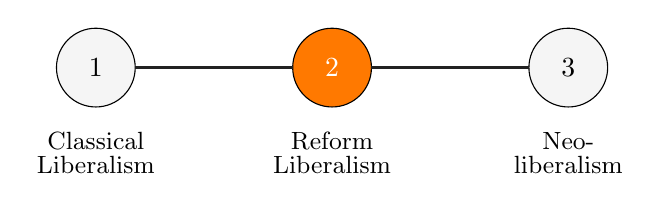
\begin{tikzpicture}
\node[draw, circle, fill=titangray, minimum size=1cm] at (0,0) {1};
\node[draw, circle, fill=titanorange, text=white, minimum size=1cm] at (3,0) {2};
\node[draw, circle, fill=titangray, minimum size=1cm] at (6,0) {3};

\draw[thick, titantext] (0.5,0) -- (2.5,0);
\draw[thick, titantext] (3.5,0) -- (5.5,0);

\node[below] at (0,-0.7) {\small Classical};
\node[below] at (0,-1.0) {\small Liberalism};
\node[below] at (3,-0.7) {\small Reform};
\node[below] at (3,-1.0) {\small Liberalism};
\node[below] at (6,-0.7) {\small Neo-};
\node[below] at (6,-1.0) {\small liberalism};
\end{tikzpicture}
\end{center}

\vspace{0.5cm}

\begin{block}{Reform Liberalism}
Emerges in response to industrialization; advocates for government intervention to address inequality and promote welfare

\vspace{0.3cm}
\textcolor{mediumblue}{\textit{Early - Mid 20th Century}}
\end{block}

\end{frame}

% Neoliberalism
\begin{frame}
\frametitle{The Evolution of Liberalism}

\begin{center}
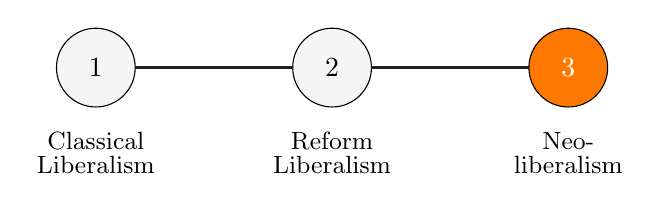
\begin{tikzpicture}
\node[draw, circle, fill=titangray, minimum size=1cm] at (0,0) {1};
\node[draw, circle, fill=titangray, minimum size=1cm] at (3,0) {2};
\node[draw, circle, fill=titanorange, text=white, minimum size=1cm] at (6,0) {3};

\draw[thick, titantext] (0.5,0) -- (2.5,0);
\draw[thick, titantext] (3.5,0) -- (5.5,0);

\node[below] at (0,-0.7) {\small Classical};
\node[below] at (0,-1.0) {\small Liberalism};
\node[below] at (3,-0.7) {\small Reform};
\node[below] at (3,-1.0) {\small Liberalism};
\node[below] at (6,-0.7) {\small Neo-};
\node[below] at (6,-1.0) {\small liberalism};
\end{tikzpicture}
\end{center}

\vspace{0.5cm}

\begin{block}{Neoliberalism}
Reacts to perceived inefficiencies of the welfare state; prioritizes market solutions with reduced government roles

\vspace{0.3cm}
\textcolor{mediumblue}{\textit{Late 20th Century - Present}}
\end{block}

\vspace{0.5cm}
\centering
This progression reflects ongoing debates about liberty, equality, and the proper role of the state.

\end{frame}

% Why Political Theory and Public Policy
\begin{frame}
\frametitle{Why Political Theory and Public Policy?}

\begin{columns}
\begin{column}{0.48\textwidth}
\begin{block}{1. Foundation}
\pause
Political theory provides a foundation for understanding governance and policy
\end{block}

\vspace{0.3cm}

\begin{block}{3. Integration}
\pause
Together, they inform how we think about and address public issues
\end{block}
\end{column}

\begin{column}{0.48\textwidth}
\begin{block}{2. Application}
\pause
Public policy applies theory to real-world problems and solutions
\end{block}

\vspace{0.3cm}

\begin{block}{4. Framework}
\pause
Reveal fundamental beliefs about the state that frame policy debates
\end{block}
\end{column}
\end{columns}

\end{frame}

% Reflection Activity
\begin{frame}
\frametitle{Reflection Activity}
\framesubtitle{Consider how different political theories might approach the same policy problem.}

\begin{block}{Example: Climate Change Policy}
\begin{columns}
\begin{column}{0.48\textwidth}
\textbf{Classical Liberal Approach}
\begin{itemize}
\item Market-based solutions
\item Property rights protection
\item Limited regulation
\end{itemize}
\end{column}

\begin{column}{0.48\textwidth}
\textbf{Reform Liberal Approach}
\begin{itemize}
\item Government intervention
\item Regulatory frameworks
\item Public investment
\end{itemize}
\end{column}
\end{columns}
\end{block}

\end{frame}

% Conclusion
\begin{frame}
\frametitle{Key Takeaways}

\begin{block}{}
\begin{itemize}
\item \textbf{Historical Evolution:} Political thought has evolved over centuries, shaping how we understand government's role
\item \textbf{Competing Values:} Different theories emphasize different values (liberty, equality, community)
\item \textbf{Modern Framework:} Liberalism in its various forms provides the framework for most contemporary policy debates
\item \textbf{Foundation for Policy:} These theories guide how we identify problems and propose solutions
\end{itemize}
\end{block}

\pause
\vspace{1cm}
\begin{center}
\textbf{Coming Up Next}

In Part 3, we'll explore policy as a tool for pursuing the common good and expressing societal values.
\end{center}

\end{frame}

\end{document}
